% Drop this file and the figures/ folder into the root of your LaTeX project.
% Select draft.tex as the main document. No Python or dataset files are needed.
\documentclass{article}
\IfFileExists{PRIMEarxiv.sty}{\usepackage{PRIMEarxiv}}{\usepackage[margin=1in]{geometry}}
\usepackage[utf8]{inputenc}
\usepackage[T1]{fontenc}
\usepackage{hyperref,url,booktabs,amsfonts,nicefrac,microtype}
\usepackage{fancyhdr,graphicx,amsmath,xcolor,amsthm,amssymb}
\graphicspath{{figures/}}
\newtheorem{proposition}{Proposition}
\newtheorem{corollary}{Corollary}
\newcommand{\kc}[1]{\textcolor{red}{KC: #1}}
\providecommand{\keywords}[1]{\par\smallskip\noindent\textbf{Keywords:} #1}
\providecommand{\AND}{\end{tabular}\par\vspace{1em}\begin{tabular}[t]{c}}
\providecommand{\And}{\and}
\IfFileExists{PRIMEarxiv.sty}{}{\renewcommand{\And}{\and}}
\pagestyle{fancy}
\fancyhf{}
\fancyfoot[C]{\thepage}
\renewcommand{\headrulewidth}{0pt}
\renewcommand{\topfraction}{0.9}
\renewcommand{\textfraction}{0.1}
\title{A Neural Dirichlet-Neumann Approach for Learning Euler Equation Flows}
\author{
  Jonathan Ma\\
  Department of Mathematics\\
  University of Delaware\\
  \texttt{johnma@udel.edu}
  \AND
  Samuel Zheng\\
  Affiliation\\
  Address\\
  \texttt{email}
  \And
  Coauthor\\
  Affiliation\\
  Address\\
  \texttt{email}
  \And
  Ke Chen\\
  Department of Mathematics\\
  University of Delaware\\
  \texttt{kechen@udel.edu}
}
\date{}
\begin{document}
\maketitle
\thispagestyle{empty}

\begin{abstract}
\textcolor{blue}{Abstract to be completed.}
\end{abstract}
\keywords{Water waves; Dirichlet--Neumann operator; neural operators}

\section{Introduction}
\label{sec:intro}
\textcolor{blue}{More needs to be added to introduction.}

\paragraph{Governing Equations \& Hamiltonian Formulation}
\textcolor{blue}{Obviously we should refine this portion later.}
We consider the evolution of a free surface on top of a two-dimensional fluid
under the influence of gravity. We let $x$ denote our horizontal direction,
and $y$ denote our vertical direction, and $t$ denote time. We assume periodic
boundary conditions on the horizontal, with domain length $L>0$.
Let $y=\eta(x,t)$ represent our free surface. We fix an impermeable bottom
at a constant depth $y=-h$. We assume the fluid is incompressible, inviscid,
and that its flow is irrotational, so that the fluid velocity is given by
$u=\nabla\varphi$, and its velocity potential $\varphi$ satisfies Laplace's
equation:
\begin{equation}
    \Delta\varphi=0,
\end{equation}
in the fluid region bounded below by the bottom at $y=-h$, and above by the
free surface defined by $\eta(x,t)$. We assume the boundary conditions
\begin{equation}
\begin{aligned}
    \varphi_y &= 0, &&\text{on }y=-h,\\
    \eta_t+\nabla_x\eta\cdot\nabla_x\varphi-\varphi_y &= 0,
      &&\text{on }y=\eta,\\
    \varphi_t+\frac12|\nabla\varphi|^2+g\eta &= 0,
      &&\text{on }y=\eta,
\end{aligned}
\label{eq:euler-system}
\end{equation}
where $g$ denotes the acceleration due to gravity.
We reduce the dimensionality of the classical potential flow formulation
of the Euler equation problem by introducing the Dirichlet--Neumann operator
(DNO), which takes Dirichlet data $\xi(x,t)=\varphi(\eta(x,t),t)$ and gives
the corresponding Neumann data, i.e., the normal velocity at the free surface.
The DNO $G$ satisfies
\[
    G(\eta)\xi=(-\nabla_x\eta,1)^\top\cdot\nabla\varphi|_{y=\eta}.
\]
The system is Hamiltonian in $\eta,\xi$, with
\begin{equation}
    H(\eta,\xi)=\frac12\int_\Omega[\xi G(\eta)\xi+g\eta^2],dx.
    \label{eq:hamiltonian}
\end{equation}
Using the fact that
\begin{equation}
    \eta_t=\frac{\delta H}{\delta\xi},\qquad
    \xi_t=-\frac{\delta H}{\delta\eta},
    \label{eq:hamiltons-equations}
\end{equation}
we can write the system \eqref{eq:euler-system} as
\begin{equation}
\begin{aligned}
    \eta_t &= G(\eta)\xi,\\
    \xi_t &= -g\eta-\frac12\xi_x^2
      +\frac{(G(\eta)\xi+\eta_x\xi_x)^2}{2(1+\eta_x^2)}.
\end{aligned}
\label{eq:hamiltonian-system}
\end{equation}
Throughout this manuscript, we note that the operator $G(\eta)$ implicitly
depends on $h$. When it is noteworthy, we note this dependence by writing the
DNO as $G(\eta;h)$. For each admissible surface $\eta$, the operator $G(\eta)$
is linear in its Dirichlet argument $\xi$, self-adjoint, and positive
semidefinite; it is positive definite after restriction to an appropriate
mean-zero space.
The Hamiltonian $H$ of our system is invariant to time. In addition to being
vital as a stability check for our classical algorithms, we will make use of
energy conservation to increase the stability of our neural network models.

\subsection{Related Work}

\subsection{Contribution}
The primary objective of this work is to construct a neural approximation
of the water-wave DNO whose evaluation is independent of the Craig--Sulem
truncation order $M$, while retaining properties needed for reliable time
integration. In particular, the proposed method is designed to achieve
accurate DNO evaluation across several challenging solution classes,
approximate Hamiltonian conservation, structural consistency, and stable
long-time trajectories. The intended principal comparison is with a vanilla
FNO trained only with the data-inconsistency loss, for which small one-step
prediction errors need not imply structure-preserving or stable dynamics.
\textcolor{blue}{The comparison with a vanilla FNO remains to be completed.}
Computational cost is examined as a practical consequence of the
$M$-independent representation, rather than as the principal contribution.

\section{Problem Setup}
We now describe methods for solving the water wave equations in terms of
solving for the DNO.

\subsection{Forward Problem Solver}
\paragraph{Craig--Sulem Series}
\textcolor{blue}{Add citations later.}
It is known that if $\eta$ is Lipschitz, then $G$ is analytic in $\eta$,
hence $G$ has a convergent Taylor series. We write
\begin{equation}
    G(\eta)=\sum_{i\geq0}G_i(\eta),
    \label{eq:cs}
\end{equation}
where $G_i$ is the $i$th homogeneous term in the Taylor expansion of $G$.
It can be shown that each term $G_i$ can be calculated using an explicit
recursion formula with base case $G_0=|D_x|\tanh(h|D_x|)$, where
$D_x=-i\nabla_x$, and $i$ is the imaginary unit. We note that $G_0$ is thus
independent of the surface shape $\eta$. By use of dynamic programming and
the fast Fourier transform, it can be shown that the time complexity of
calculating the $M$th polynomial $G_M$ is $\Theta(M^2N\log N)$, where $N$
is the spatial discretization dimension. Xu and Guyenne make use of this
recursive method of calculating $G$ up to the $M$th Taylor term in
[\textcolor{blue}{cite}] to solve the water wave problem. The details of this
algorithm are in the appendix.

\paragraph{Numerical Methods for CS Series}
\textcolor{blue}{Add typical method for calculating the DNO. Add challenges
of calculating DNO.}

\paragraph{Time Integrator}
Following Xu and Guyenne, we employ an implicit symplectic scheme to solve
our time stepping PDE problem. Details in appendix.
\textcolor{green!50!black}{Sam}

\subsection{Learning Problem}
\textcolor{blue}{Describe learning the DNO operator using a parametrized
model, and a dataset $\mathcal D$ and loss $\mathcal L$. Need to emphasize
that the target operator is depth dependent and the PDE is time dependent.
Want to learn many classes of initial conditions and maintain long-time
stability.}

\paragraph{Deep Learning / Scientific Machine Learning}
Deep learning methods have recently seen success in being incorporated into
solutions for scientific problems, especially those governed by partial
differential equations. This has given rise to the field of Scientific
Machine Learning. Practitioners leverage the well-known universal
approximation results of deep neural networks to model unknown target
functions using data. When extended to the appropriate domains and function
spaces of partial differential equation solutions, this is often referred
to as operator learning.
Given the goal of replacing the costly computation of the DNO with a
cheap-to-evaluate and accurate neural surrogate, we require describing a
parametric neural network model $G_\theta$, a dataset $\mathcal D$ to learn
from, and a loss function $\mathcal L$ to enforce consistency of our
parametric model with the target operator $G$. We describe our parametric
family of models in Section~\ref{sec:architecture}, the construction of
$\mathcal D$ in Section~\ref{sec:DataGen}, and our choice of $\mathcal L$
in Section~\ref{section:loss-fn}.

\paragraph{Operator Learning}
Operator learning is broadly characterized by methods for approximating
mappings between Hilbert or Banach spaces. In practice, this is achieved by
designing methods of approximation which are invariant to choice of
discretization of the domain $\Omega$. We achieve this by using a Fourier
Neural Operator (FNO) backbone.

\section{Proposed Method}
We propose a method for solving the water wave equations by approximating
the DNO. Additionally, we demonstrate that simply approximating the DNO
pointwise is insufficient for maintaining stability in the downstream
numerical PDE task. Thus we provide several physics-informed methods for
ensuring that the learned DNO provides the necessary stability for PDE
simulation.

\subsection{Designing a Loss Function}
\label{section:loss-fn}
We teach our model the law of the DNO operator by penalizing the following
loss:
\begin{equation}
    \mathcal L_{\mathrm{DNO}}=
    \alpha_1\mathcal L_{L^2}+\alpha_2\mathcal L_{\mathrm{MB}}
    +\alpha_3\mathcal L_{\mathrm{TG}}+\alpha_4\mathcal L_{\mathrm{HD}},
\end{equation}
where the coefficients $\alpha_i$ are a convex combination determined through
hyperparameter search. The loss $\mathcal L_{L^2}$ is the ordinary $L^2$
loss, calculated spectrally. \kc{New notations should be defined.}
The last three terms of our aggregate loss are each derived from the
Hamiltonian of our system, helping ensure the learned dynamics of our
network are consistent with physics. Each loss is carefully ablated.

\subsection{Hamiltonian Mode-Balancing Penalty}
\textcolor{blue}{Need to numerically show that during water wave simulation
it is possible that certain modes tend to zero or certain modes completely
dominate the output.}
As we are learning our operator chiefly in Fourier space, and using a
spectral solver in the downstream PDE simulation, we aim to ensure that
our learned operator respects the evolution of each active Fourier mode in
a given instantiation of our time-stepping PDE. A key challenge in ensuring
this is disallowing certain modes to dominate the evolution.
\textcolor{blue}{Add supporting references.}
We show that a single-step loss which penalizes long-term mismatches in
Fourier mode activity can be derived from the Hamiltonian of our problem.
We begin by deriving a quadratic approximation to our Hamiltonian
\eqref{eq:hamiltonian}. Define $F(\varepsilon):=G(\varepsilon\eta)\xi$,
for fixed $\eta,\xi$, and $\varepsilon>0$. Applying a Taylor expansion on
$F$ about zero gives
\begin{equation}
    F(\varepsilon)=F(0)+\varepsilon F'(0)+\mathcal O(\varepsilon^2).
\end{equation}
Perturbing \eqref{eq:hamiltonian} by $\varepsilon$,
\begin{align}
    H(\varepsilon\eta,\varepsilon\xi)
    &=\frac12\int_\Omega\varepsilon\xi\cdot
        G(\varepsilon\eta)\varepsilon\xi\,dx
      +\frac g2\int_\Omega\varepsilon^2\eta^2\,dx\\
    &=\frac12\int_\Omega\varepsilon^2\xi
      [F(0)+\varepsilon F'(0)+\mathcal O(\varepsilon^2)]\xi\,dx
      +\frac g2\int_\Omega\varepsilon^2\eta^2\,dx\\
    &=\varepsilon^2\left(\frac12\int_\Omega\xi F(0)
        +\frac g2\int_\Omega\eta^2\,dx\right)
      +\varepsilon^3\left(\frac12\int_\Omega F'(0)\right)
      +\mathcal O(\varepsilon^4).
\end{align}
Therefore the quadratic Hamiltonian is
\begin{equation}
    H_2(\eta,\xi)=\frac12\int_\Omega[\xi G(0)\xi+g\eta^2],dx.
    \label{eq:quadratic-H}
\end{equation}
The Fourier symbol of the flat-surface DNO, $G(0)$, has known form:
\begin{equation}
    \widehat{G(0)\xi}_k=|k|\tanh(h|k|)\widehat\xi_k.
\end{equation}
Thus by using Parseval's theorem, one may calculate that for any
$\eta,\xi$, $H_2(\eta,\xi)=\sum_kH_2(\eta,\xi)_k$, where
\begin{equation}
    H_2(\eta,\xi)_k=\frac12
    \left(|k|\tanh(h|k|)|\widehat\xi_k|^2+g|\widehat\eta_k|^2\right).
\end{equation}
Plugging \eqref{eq:quadratic-H} into \eqref{eq:hamiltons-equations} yields
the linearized system
\begin{equation}
    \eta_t^{\mathrm L}=G(0)\xi,\qquad \xi_t^{\mathrm L}=-g\eta.
\end{equation}
Taking the Fourier transform yields, for nonzero modes $k$,
\begin{equation}
    \partial_t\widehat{\eta_k^{\mathrm L}}=\widehat{G(0)\xi_k},
    \qquad \partial_t\widehat{\xi_k^{\mathrm L}}=-g\widehat\eta_k.
\end{equation}
Differentiating the first equation once more in time,
\begin{align}
    \partial_{tt}\widehat{\eta_k^{\mathrm L}}
    &=\widehat{G(0)}_k\partial_t\widehat\xi_k\\
    &=-g\widehat{G(0)}_k\widehat{\eta_k^{\mathrm L}}.
\end{align}
Define $\omega_k^2:=g\widehat{G(0)}_k$, then note that
\begin{equation}
    \partial_{tt}\widehat{\eta_k^{\mathrm L}}
       +\omega_k^2\widehat{\eta_k^{\mathrm L}}=0
\end{equation}
is a harmonic oscillator with frequency $\omega_k$, whose amplitude is
\begin{equation}
    A_k^2=|\widehat{\eta_k^{\mathrm L}}|^2
      +\frac{|\partial_t\widehat{\eta_k^{\mathrm L}}|^2}{\omega_k^2}.
\end{equation}
Furthermore, this quantity is invariant to time:
\begin{align*}
\frac{d}{dt}A_k^2
&=\partial_t\widehat\eta_k^{\mathrm L}\,
    \overline{\widehat\eta_k^{\mathrm L}}
  +\widehat\eta_k^{\mathrm L}\,
    \partial_t\overline{\widehat\eta_k^{\mathrm L}}\\
&\quad+\frac1{\omega_k^2}
  \left(\partial_{tt}\widehat\eta_k^{\mathrm L}\,
    \partial_t\overline{\widehat\eta_k^{\mathrm L}}
  +\partial_t\widehat\eta_k^{\mathrm L}\,
    \partial_{tt}\overline{\widehat\eta_k^{\mathrm L}}\right)\\
&=\partial_t\widehat\eta_k^{\mathrm L}\,
    \overline{\widehat\eta_k^{\mathrm L}}
  +\widehat\eta_k^{\mathrm L}\,
    \partial_t\overline{\widehat\eta_k^{\mathrm L}}\\
&\quad+\frac1{\omega_k^2}
  \left(\omega_k^2\widehat\eta_k^{\mathrm L}\,
    \partial_t\overline{\widehat\eta_k^{\mathrm L}}
  +\omega_k^2\partial_t\widehat\eta_k^{\mathrm L}\,
    \overline{\widehat\eta_k^{\mathrm L}}\right)\\
&=0.
\end{align*}
\textcolor{blue}{We use this quantity to quantify the scale of the $k$th
Fourier mode of the target $G(\eta)\xi$, for fixed $\eta,\xi$.}

\subsection{Tangent-Gain Penalty}
For fixed $\eta,\xi$, write the error of our model $G_\theta$ against $G$ by
$\mathcal E=G_\theta(\eta)\xi-G(\eta)\xi$. If we assume that for some
$c>0$ our wave has a transporting profile, $G(\eta)\xi:=-c\eta_x$, then,
assuming $G_\theta(\eta)\xi\approx(1+\varepsilon)G(\eta)\xi$, we find
$\mathcal E\approx-\varepsilon c\eta_x$, which is an accelerative error in
the translating direction. We empirically find that when simulating the
water wave equations using a na\"ive neural surrogate with certain initial
wave profiles, translating error dominates the error accumulated.
\textcolor{blue}{Add a small numerical experiment to support this.}
We thus provide a simple loss which targets general potential translation
error accumulated during the simulation of the water wave PDE.
For fixed $x$, $\eta$, and $a>0$, the velocity of the translating operator
$T_a(\eta):=\eta(x-a)$ is $-\eta_x$. Let $P_{\eta_x}$ be the $L^2$
projection operator onto $\operatorname{span}\{\eta_x\}$. As before, let
$\mathcal E=G_\theta(\eta)\xi-G(\eta)\xi$. We would like to penalize
\begin{equation}
    \frac{\|P_{\eta_x}\mathcal E\|^2}{\|\eta\|_2^2}
    =\frac{|\langle\mathcal E,\eta_x\rangle|^2}
       {\|\eta\|_2^2\|\eta_x\|_2^2},
    \label{eq:tg}
\end{equation}
where we divide by the square norm of $\eta$ as is practice in deep learning
to maintain scale invariance of our loss function.
In practice, a target wave profile may have more than one translating
component, with varying speeds, which motivates deriving a localized version
of \eqref{eq:tg}. We first define the periodic Gaussian kernel
\[
K_\sigma(x-y):=\frac1{\sqrt{2\pi\sigma^2}}
\sum_{m\in\mathbb Z}\exp\left(-\frac{(x-y+mL)^2}{2\sigma^2}\right),
\]
for $x,y\in\mathbb T_L$ and $\sigma^2>0$ the variance/localization parameter
of the kernel. We then define the following averaging operator:
\[
    (B_\sigma f)(x):=\int_0^L K_\sigma(x-y)f(y)\,dy.
\]
For $k_n=2\pi n/L$, the $n$th Fourier series coefficient of our kernel is
$\widehat K_{\sigma,n}=L^{-1}\exp(-\sigma^2k_n^2/2)$. For a periodic
function $f(x)=\sum_{n\in\mathbb Z}\widehat f_n\exp(ik_nx)$, by the
convolution theorem,
\[
    \widehat{(B_\sigma f)_n}=\exp(-\sigma^2k_n^2/2)\widehat f_n.
\]
The above Fourier multiplier form of $B_\sigma$ is useful for us as
numerically we calculate this convolution spectrally rather than physically.
Upon defining our averaging operator, we replace our $L^2$ inner product
with our localized inner product
$\langle f,g\rangle_{\sigma,x}=\int_{\mathbb T_L}K_\sigma(x,y)f(y)g(y)\,dy$.
We repeat the above step of projecting the error $\mathcal E$ onto the span
of $\eta_x$ under our new weighted inner product using the projection
operator $P_{\eta_x}^{\sigma,x_0}$, where we emphasize the dependence on
the fixed reference point $x_0$:
\[
\frac{\|P_{\eta_x}^{\sigma,x_0}\mathcal E\|^2_{\sigma,x_0}}
     {\|\eta\|_2^2}
=\frac{|\langle\mathcal E,\eta_x\rangle_{\sigma,x_0}|^2}
     {\|\eta\|_2^2\|\eta_x\|_{\sigma,x_0}^2}.
\]
Lastly, we integrate over all reference points $x_0$ to define our loss
$\mathcal L_{\mathrm{TG}}$:
\begin{equation}
    \mathcal L_{\mathrm{TG}}=\frac1{\|\eta\|_2^2}
    \int_{\mathbb T_L}\|P_{\eta_x}^{\sigma,x_0}\mathcal E\|^2_{\sigma,x_0}\,dx_0.
\end{equation}

\subsection{Hadamard Derivative}
\textcolor{blue}{Jonathan}
Intuitively learning the DNO pointwise from data is insufficient to
guarantee stability during simulation of the time-stepping PDE. Notably,
as our network only claims to be an approximation to the true DNO, even
small numerical error in its approximation will force the network to make
predictions on future states which may only necessarily be near the true
PDE trajectory. We cite the following theorem of Lannes which can help
encourage our network to be locally accurate in an appropriate manner.
\begin{proposition}
\label{prop:dno-shape-derivative}
Let $\eta$, $\xi$, and $\zeta$ be sufficiently smooth, and assume that the
fluid depth remains strictly positive. Define
\[
q=G(\eta)\xi,\qquad
B=\frac{q+\eta_x\xi_x}{1+\eta_x^2},\qquad V=\xi_x-\eta_xB.
\]
Then the map $\eta\mapsto G(\eta)\xi$ is Fr\'echet differentiable and
\[
    D_\eta G(\eta)[\zeta]\xi=-G(\eta)(\zeta B)-\partial_x(\zeta V).
\]
\end{proposition}
A proof is provided in the appendix, as well as \textcolor{blue}{citations}.
To enforce local correctness of our learned model $G_\theta$, we define
the residual of $G_\theta$ with Proposition~\ref{prop:dno-shape-derivative}:
\[
\mathcal H_\theta(\eta,\xi;\zeta)
=D_\eta G_\theta(\eta)[\zeta]\xi
 +G_\theta(\eta)(\zeta B_\theta)+\partial_x(\zeta V_\theta),
\]
where
\[
B_\theta=\frac{G_\theta(\eta)\xi+\eta_x\xi_x}{1+\eta_x^2},
\qquad V_\theta=\xi_x-\eta_xB_\theta.
\]
We approximate this Fr\'echet derivative by sampling a random direction
$\zeta$ on the unit sphere $S^{d-1}$, where $d$ is our discretization
dimension, and sampling $\varepsilon\sim\mathcal U(10^{-3},3\times10^{-3})$,
then we calculate
\[
D_\eta G_\theta(\eta)[\zeta]\xi\approx
\frac{G_\theta(\eta+\varepsilon\zeta)\xi-G_\theta(\eta)\xi}{\varepsilon}.
\]
The terms $\partial_x(\zeta V_\theta)$, $\eta_x$, and $\xi_x$ are calculated
by spectral differentiation. We then define the loss $\mathcal L_{\mathrm{HD}}$
as
\begin{equation}
\mathcal L_{\mathrm{HD}}=
\mathbb E_{\substack{\zeta\sim\mathcal U(S^{d-1})\\
\varepsilon\sim\mathcal U(10^{-3},3\times10^{-3})}}
[\mathcal H_\theta(\eta,\xi;\zeta)].
\end{equation}

\subsection{Architecture}
\label{sec:architecture}
We now describe the architectural decisions we made in defining our family
of parametric models for learning the DNO. Our network is built chiefly in
Fourier space, as a composition of learned Fourier multipliers. We show that
this allows our network to satisfy several properties of the DNO by
construction, as well as enabling the discretization invariance trait which
is desirable in operator learning.

\paragraph{CS Truncation}
The first term of \eqref{eq:cs} has a known Fourier symbol:
\begin{equation}
    \widehat{G_0\xi}_k=|k|\tanh(h|k|)\widehat\xi_k.
    \label{eq:base-case}
\end{equation}
The second term of \eqref{eq:cs}, through the known Craig--Sulem recursion,
is written
\begin{equation}
    G_1(\eta)\xi=D\cdot(\eta D\xi)-G_0(\eta G_0\xi).
\end{equation}
We thus propose to learn the following approximation:
\begin{equation}
    G(\eta)\xi\approx G_0\xi+G_1(\eta)\xi+G_\theta(\eta)\xi,
\end{equation}
where $G_\theta$ is our learned surrogate.
\textcolor{blue}{We should quantify the actual error between $G$ and
$G_0+G_1$ to give some motivation. It is of course $\mathcal O(\eta^2)$.}

\paragraph{Low Rankedness of Residual}
\textcolor{blue}{Jonathan}

\paragraph{Depth and Wavenumber Conditioning}
As mentioned in Section~\ref{sec:intro}, the DNO depends on the geometry of
the prescribed water wave problem. In our two-dimensional fluid setting,
this geometry dependence is explicit in the depth of our impermeable bottom
at depth $-h$. In addition, due to the depth dependence in the base case of
our CS recursion \eqref{eq:base-case}, the depth parameter $h$ acts
mode-by-mode on the DNO. \textcolor{blue}{Jonathan}

\paragraph{Positive Definiteness and Linearity}
As mentioned in Section~\ref{sec:intro}, for each admissible $\eta$ the target
operator $G(\eta)$ is linear in $\xi$ and positive semidefinite, which
motivates the following architectural decisions for the neural surrogate
$G_\theta$.

\subsection{Training the Neural Operator}
\textcolor{blue}{Jonathan}

\section{Numerical Experiments}
We compare the learned DNO with the Craig--Sulem (CS) reference solver.
Here $G_\theta(\eta;h)\xi$ includes both the analytic terms and the
learned correction.

\subsection{Numerical Setup and Data Generation}
\label{sec:DataGen}
\subsubsection{Wave Regimes}
We use four wave families:
\begin{enumerate}
    \item Stokes traveling waves;
    \item Tanaka solitary waves, including isolated and multiple-wave cases;
    \item JONSWAP/TMA irregular waves; and
    \item Benjamin--Feir configurations with a carrier and perturbing sidebands.
\end{enumerate}
The dataset contains 3,686,400 snapshots per family, or 14,745,600 in total.
Figure~\ref{fig:wave-regimes} shows one training snapshot from each family.

\begin{figure}[tbp]
    \centering
    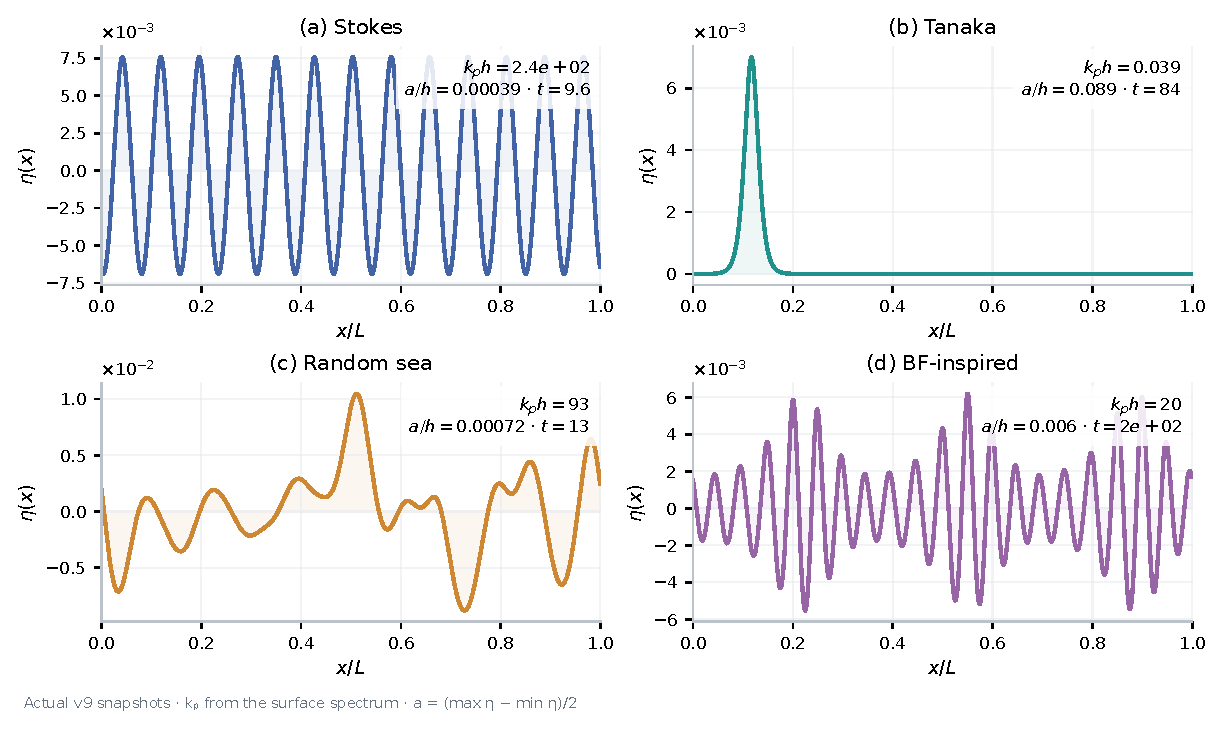
\includegraphics[width=0.98\linewidth]{01-wave-regimes.pdf}
    \caption{Training examples from the four wave families, selected near
    each family's median sampled DNO error. Here $k_p$ is the dominant
    nonzero surface wavenumber and $a=(\max\eta-\min\eta)/2$.}
    \label{fig:wave-regimes}
\end{figure}

\subsubsection{Reference Solver and Dataset Construction}
The test trajectories use a periodic domain of length
$L=2\pi$, $N_x=1024$ grid points, and gravity $g=1$. The reference DNO is
computed with Craig--Sulem order $M_{\mathrm{ref}}=6$ and padding factor
eight. Reference and learned trajectories use the same integrating-factor
Gauss--Legendre scheme, with four fixed-point iterations, time step
$\Delta t=0.01$, and a spectral cutoff at mode 128. No adaptive damping
is applied.

Entire simulations are assigned to training, validation, or test sets,
containing 11,796,720, 1,474,440, and 1,474,440 snapshots, respectively.
The one-step accuracy test samples 512 snapshots per family from each of
the training and test sets.

Trajectory tests use 32 initial conditions per family from the test set,
chosen across the sampled parameter ranges. We integrate to $T=20$ for
Stokes and JONSWAP/TMA and $T=200$ for Tanaka and Benjamin--Feir, saving
251 equally spaced states per trajectory.

\subsubsection{Implementation Details}
\label{sec:Implement}
The network has 1,342,400 parameters and is selected by validation error
after 40 training epochs. Network evaluation uses single precision; the
analytic terms, time integration, and Hamiltonian evaluation use double
precision. Timing measurements use an AMD EPYC 9124 CPU with eight logical
CPUs, excluding compilation.

\subsection{Accuracy and Structural Properties of the Learned DNO}
\label{sec:Accuracy}
\subsubsection{Relative DNO Accuracy}
For sample $j$, define
\begin{equation}
e_G^{(j)}=
\frac{\|G_\theta(\eta^{(j)};h^{(j)})\xi^{(j)}
       -G(\eta^{(j)};h^{(j)})\xi^{(j)}\|_{L^2}}
     {\|G(\eta^{(j)};h^{(j)})\xi^{(j)}\|_{L^2}}.
\label{eq:dno-relative-error}
\end{equation}
Figure~\ref{fig:dno-class-errors} compares the learned DNO with the stored
reference targets, grouped by wave family and relative depth $k_ph$.

\begin{figure}[tbp]
    \centering
    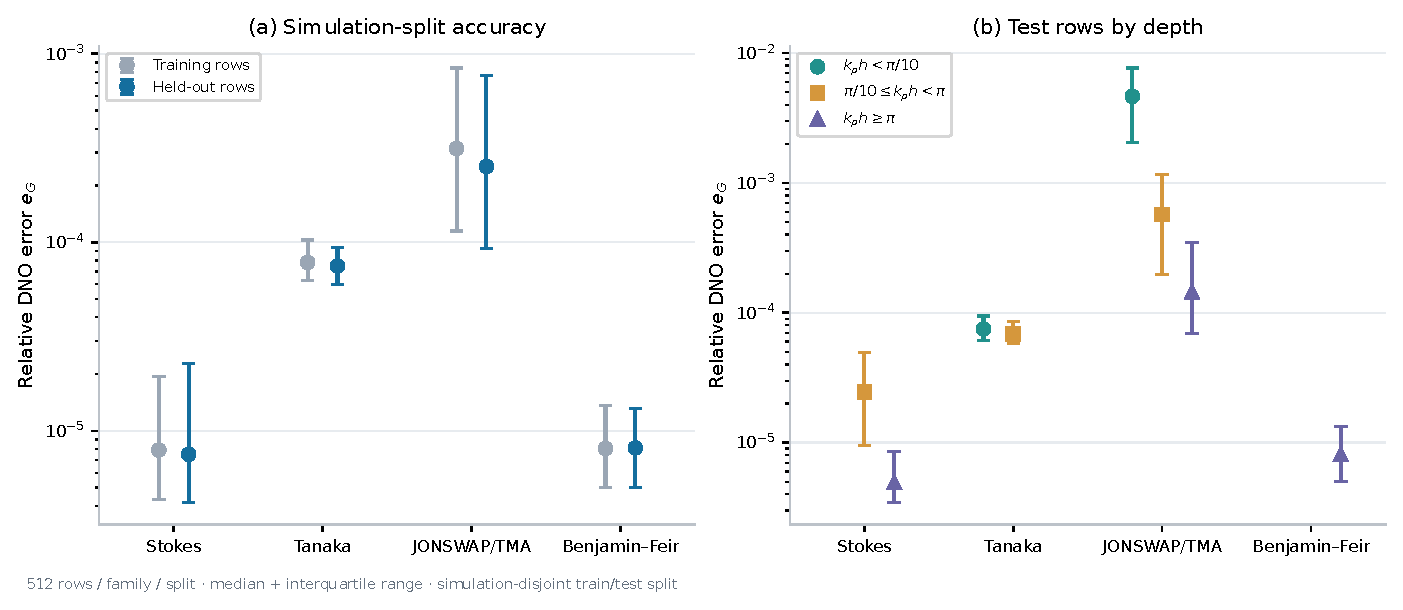
\includegraphics[width=0.98\linewidth]{02-dno-class-errors.pdf}
    \caption{Relative $L^2$ DNO errors for 512 sampled snapshots per family
    per split. Left: training and test medians with interquartile ranges.
    Right: test errors grouped by $k_ph<\pi/10$,
    $\pi/10\leq k_ph<\pi$, and $k_ph\geq\pi$; empty groups are omitted.}
    \label{fig:dno-class-errors}
\end{figure}

\subsubsection{Linearity and Positive Semidefiniteness}
For fixed $(\eta,h)$, Dirichlet data $\xi_1,\xi_2$, and scalars $a,b$, define
\begin{equation}
e_{\mathrm{lin}}=
\frac{\|G_\theta(\eta;h)(a\xi_1+b\xi_2)
       -aG_\theta(\eta;h)\xi_1-bG_\theta(\eta;h)\xi_2\|_{L^2}}
     {|a|\|G_\theta(\eta;h)\xi_1\|_{L^2}
       +|b|\|G_\theta(\eta;h)\xi_2\|_{L^2}}.
\label{eq:linearity-residual}
\end{equation}
We perform 100 independent trials per family. The surface-depth pair and
two Dirichlet inputs are drawn independently from training snapshots of
that family; the inputs are centered, and $a,b$ are sampled independently
from $\mathcal U(-1,1)$. Mean linearity residuals range from
$3.37\times10^{-6}$ to $1.50\times10^{-4}$ across the four families with
single-precision network evaluation.

Because constant Dirichlet data belong to the DNO nullspace, its quadratic
form is positive semidefinite on the full space. For
$\widetilde\xi=\xi-L^{-1}\int_0^L\xi(x)\,dx$, define
\begin{equation}
q_\theta(\eta,\widetilde\xi;h)=
\frac{\langle\widetilde\xi,G_\theta(\eta;h)\widetilde\xi\rangle_{L^2}}
     {\|\widetilde\xi\|_{L^2}^2}.
\label{eq:positivity-statistic}
\end{equation}
On 100 independently sampled matched training snapshots per family, no
quadratic form falls below $-\tau$, with $\tau=10^{-10}$. This finite
sample test is not a proof of positive semidefiniteness of the learned
operator.

\subsection{Trajectory Accuracy and Long-Time Stability}
\label{sec:TrajectoryAccuracy}
Define the trajectory errors by
\begin{equation}
e_\eta(t)=\frac{\|\eta_\theta(t)-\eta_{\mathrm{CS}}(t)\|_{L^2}}
                   {\|\eta_{\mathrm{CS}}(t)\|_{L^2}},\qquad
e_\xi(t)=\frac{\|\xi_\theta(t)-\xi_{\mathrm{CS}}(t)\|_{L^2}}
                 {\|\xi_{\mathrm{CS}}(t)\|_{L^2}}.
\label{eq:state-relative-errors}
\end{equation}
Potential fields are compared in the mean-zero gauge. For saved times
$t_0,\ldots,t_{N_t}$, the surface trajectory error is
\begin{equation}
E_{\eta,\mathrm{traj}}=
\left(\frac{\sum_{n=0}^{N_t}\|\eta_\theta(t_n)-\eta_{\mathrm{CS}}(t_n)\|_{L^2}^2}
{\sum_{n=0}^{N_t}\|\eta_{\mathrm{CS}}(t_n)\|_{L^2}^2}\right)^{1/2},
\label{eq:eta-trajectory-error}
\end{equation}
with $E_{\xi,\mathrm{traj}}$ defined analogously. The terminal errors are
$e_\eta(T)$ and $e_\xi(T)$.

\subsubsection{Overall Trajectory Accuracy and Stability}
Figure~\ref{fig:trajectory-errors} summarizes all 128 test trajectories.
All saved states are finite and have positive fluid depth.

\begin{figure}[tbp]
    \centering
    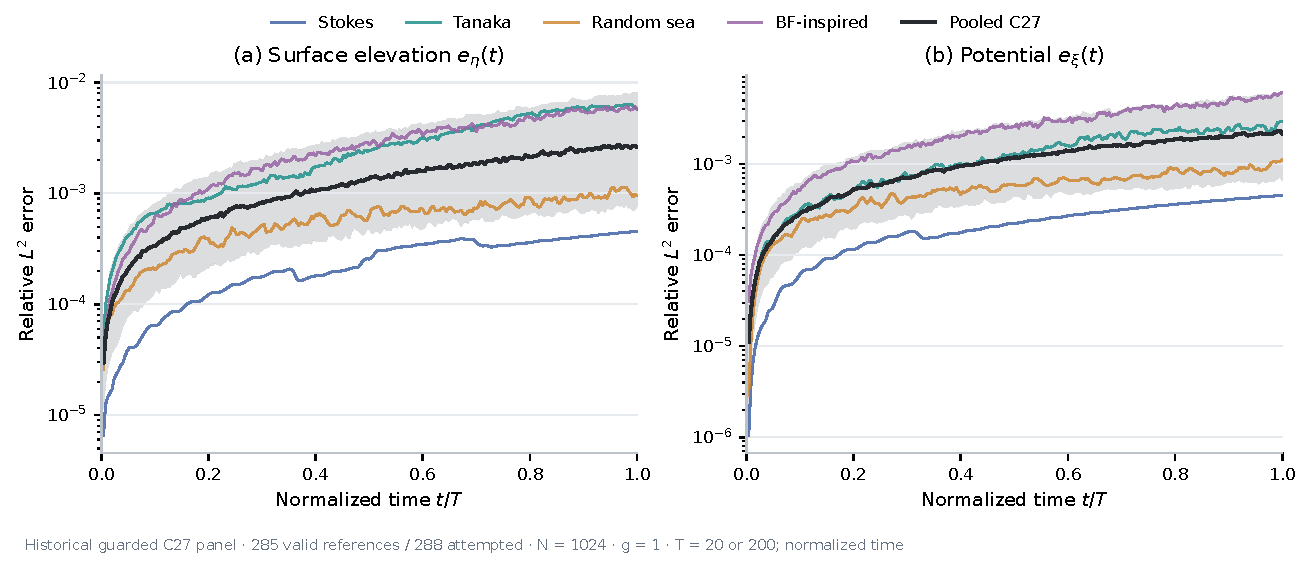
\includegraphics[width=0.98\linewidth]{03-trajectory-errors.pdf}
    \caption{Relative surface and potential errors for 128 test trajectories,
    32 per family. Black curves and shading show the overall median and
    interquartile range; colored curves show family medians. Time is
    normalized by each family's integration horizon $T$.}
    \label{fig:trajectory-errors}
\end{figure}

\subsubsection{Regime-Specific Physical Accuracy}
\paragraph{Traveling Stokes and Tanaka Waves}
For a periodic traveling wave, define the translation error by
\begin{equation}
\Delta x(t)=\underset{s\in[-L/2,L/2)}{\operatorname{argmin}}
\|\eta_\theta(\cdot,t)-\eta_{\mathrm{CS}}(\cdot-s,t)\|_{L^2}.
\label{eq:translation-error}
\end{equation}
The translation-aligned profile error is
\begin{equation}
e_{\eta,\mathrm{align}}(t)=
\frac{\|\eta_\theta(\cdot,t)-\eta_{\mathrm{CS}}(\cdot-\Delta x(t),t)\|_{L^2}}
{\|\eta_{\mathrm{CS}}(\cdot,t)\|_{L^2}}.
\label{eq:aligned-profile-error}
\end{equation}
Figure~\ref{fig:traveling-wave-accuracy} separates phase drift from profile
distortion for Stokes and single-wave Tanaka cases near their respective
median terminal errors. Alignment uses Fourier interpolation; Stokes
displacements are unwrapped modulo one carrier wavelength.

\begin{figure}[tbp]
    \centering
    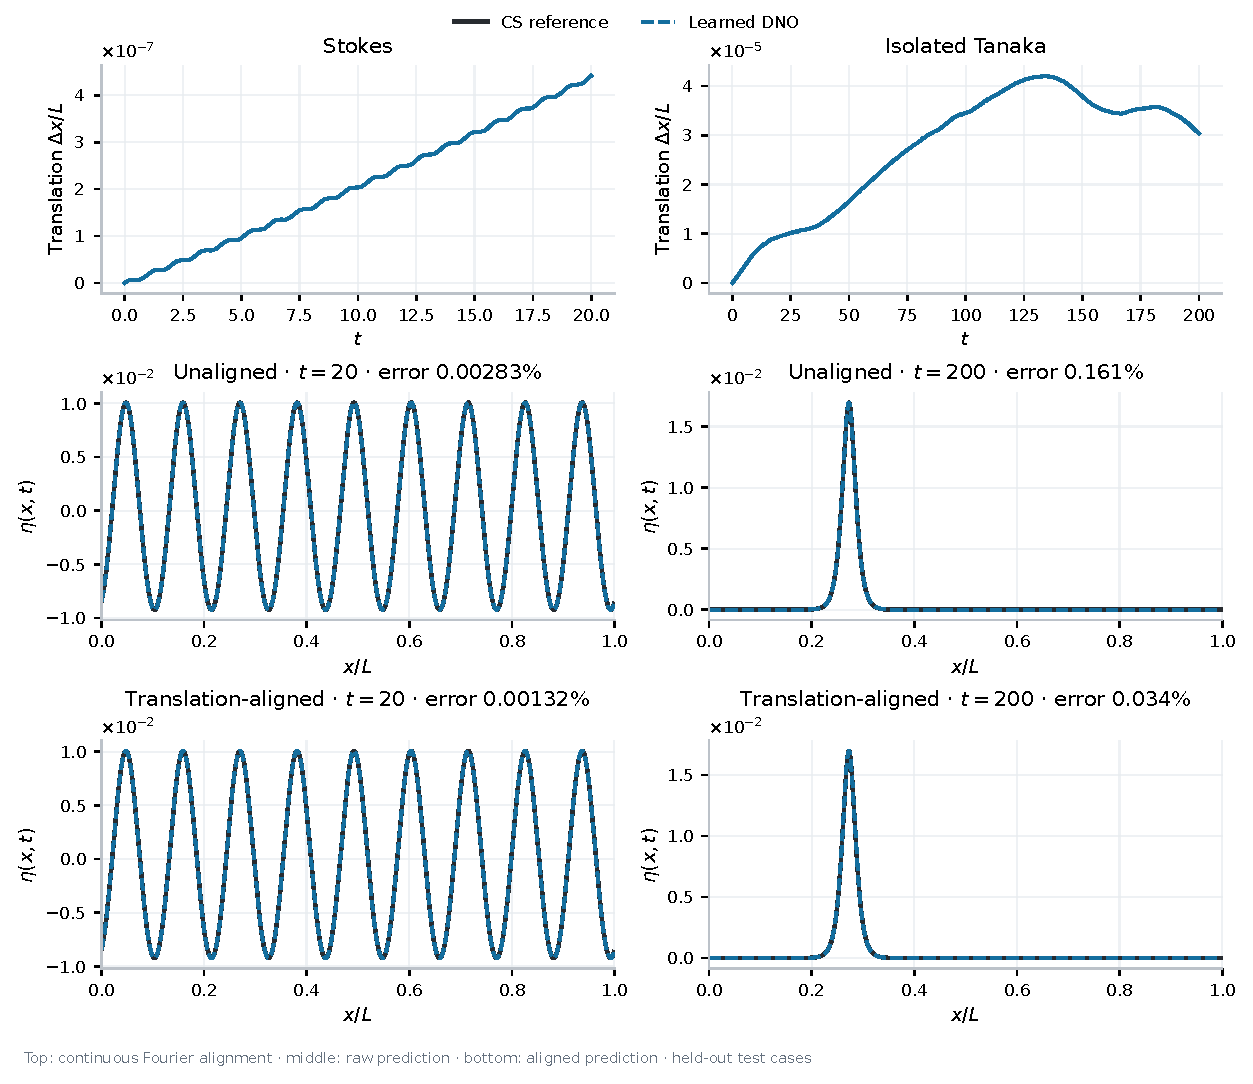
\includegraphics[width=0.98\linewidth,height=0.68\textheight,keepaspectratio]{04-traveling-wave-accuracy.pdf}
    \caption{Traveling Stokes and Tanaka waves. Top: displacement error
    $\Delta x/L$. Middle: reference and learned profiles. Bottom: profiles
    after translation alignment. Both unaligned and aligned errors are reported.}
    \label{fig:traveling-wave-accuracy}
\end{figure}

\paragraph{Tanaka-Wave Interactions}
For the intended collision study, define the collision time as the time
of minimum periodic separation between two tracked crests, and set
\begin{equation}
e_{\mathrm{coll}}=
\frac{|T_{\mathrm{coll},\theta}-T_{\mathrm{coll},\mathrm{CS}}|}
{T_{\mathrm{coll},\mathrm{CS}}}.
\label{eq:collision-time-error}
\end{equation}
Figure~\ref{fig:tanaka-collision} shows profiles around a local maximum of
reference crest amplification. Both solutions use the same fixed spatial
shift. The tracked-crest collision-time error in
\eqref{eq:collision-time-error} is not measured here.

\begin{figure}[tbp]
    \centering
    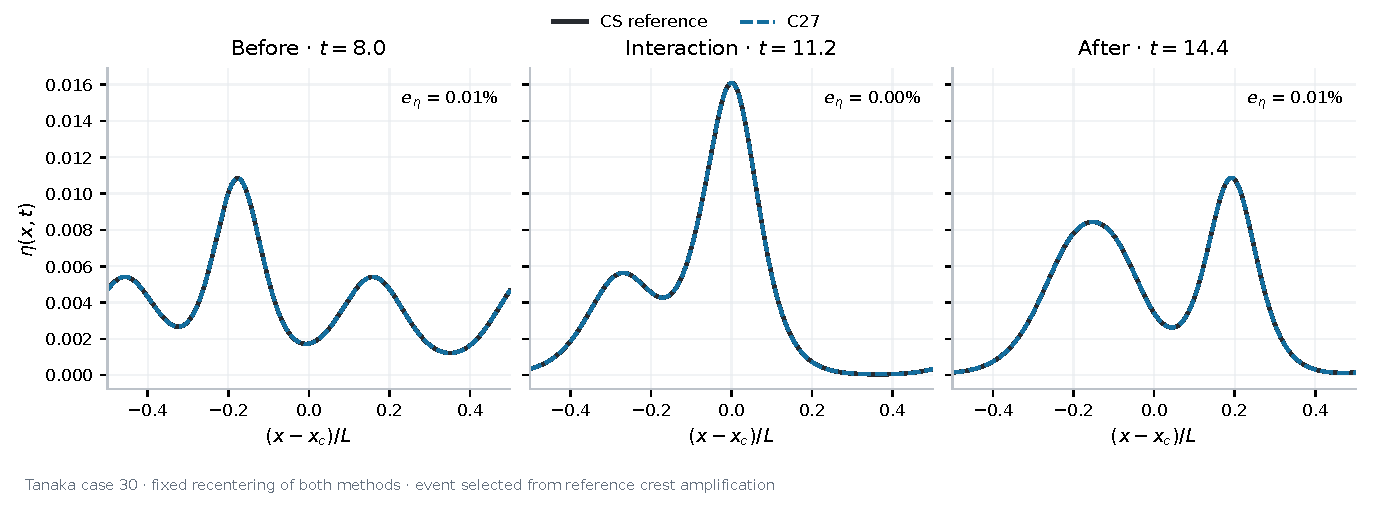
\includegraphics[width=0.98\linewidth]{05-tanaka-collision.pdf}
    \caption{A two-wave Tanaka interaction at depth $h=0.039392$.
    Reference and learned profiles are shown on identical axes at
    $t=14.4$, $17.6$, and $20.8$, with relative surface errors.}
    \label{fig:tanaka-collision}
\end{figure}

\paragraph{Benjamin--Feir and JONSWAP/TMA Waves}
For periodic wavenumbers $k=2\pi n/L$, define
\begin{equation}
\lambda_k(h)=|k|\tanh(h|k|),\qquad
\mathcal E_k(t)=\frac12\left[g|\widehat\eta_k(t)|^2
+\lambda_k(h)|\widehat\xi_k(t)|^2\right].
\label{eq:modal-energy}
\end{equation}
The normalized spectral-energy distribution and its transfer from the
initial state are
\begin{equation}
p_k(t)=\frac{\mathcal E_k(t)}{\sum_j\mathcal E_j(t)},\qquad
\Delta p_k(t)=p_k(t)-p_k(0).
\label{eq:spectral-energy-transfer}
\end{equation}
For a carrier $k_0$ with symmetric sidebands spaced by $q$, define
\begin{equation}
R_{\mathrm{sb}}(t)=
\frac{\mathcal E_{k_0-q}(t)+\mathcal E_{k_0+q}(t)}{\mathcal E_{k_0}(t)}.
\label{eq:sideband-ratio}
\end{equation}
Figure~\ref{fig:spectral-transfer} shows two held-out examples. For
Benjamin--Feir waves, we use the strongest symmetric sideband pair in the
initial spectrum. For JONSWAP/TMA, the initial peak mode $n_p$ defines
low ($0<n<0.5n_p$), peak ($0.5n_p\leq n\leq1.5n_p$), and high
($n>1.5n_p$) bands. One-sided spectra include both members of each
conjugate-mode pair.

\begin{figure}[tbp]
    \centering
    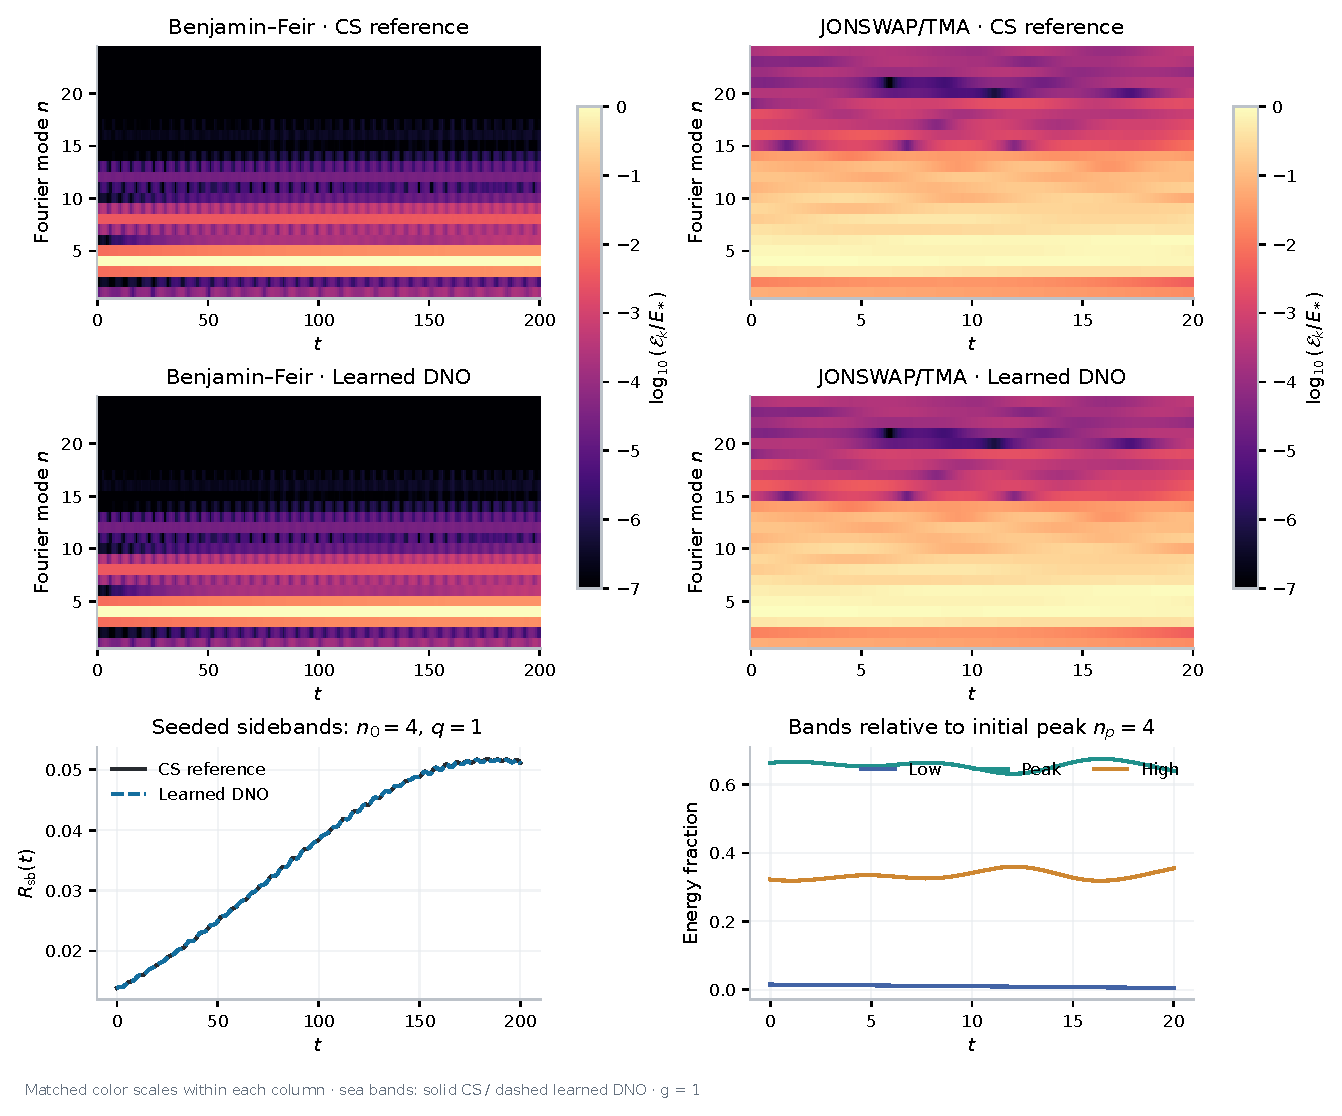
\includegraphics[width=0.98\linewidth,height=0.68\textheight,keepaspectratio]{06-spectral-transfer.pdf}
    \caption{Spectral energy for Benjamin--Feir and JONSWAP/TMA waves.
    Paired heatmaps share a color scale normalized by their joint maximum
    $E_*$. Below: sideband-to-carrier ratio and band-energy fractions.
    Solid curves denote the reference; dashed curves denote the learned DNO.}
    \label{fig:spectral-transfer}
\end{figure}

\subsection{Hamiltonian Conservation}
\label{sec:HamiltonianExperiment}
To assess physical energy independently of the learned DNO, we evaluate
the Hamiltonian of a predicted state using the reference Craig--Sulem
operator:
\begin{equation}
H_{\mathrm{ref}}^\theta(t)=\frac12\int_\Omega
\left[\xi_\theta(t)G(\eta_\theta(t);h)\xi_\theta(t)
+g\eta_\theta(t)^2\right]dx.
\label{eq:reference-evaluated-hamiltonian}
\end{equation}
The signed and absolute relative drifts are
\begin{equation}
\delta_H(t)=\frac{H_{\mathrm{ref}}^\theta(t)-H_{\mathrm{ref}}^\theta(0)}
{|H_{\mathrm{ref}}^\theta(0)|},\qquad e_H(t)=|\delta_H(t)|.
\label{eq:hamiltonian-drift}
\end{equation}
We evaluate the sixth-order reference DNO on both solutions at 26 times
per trajectory. Figure~\ref{fig:hamiltonian-drift} shows the resulting drift,
which is larger for the learned trajectories than for the reference.

\begin{figure}[tbp]
    \centering
    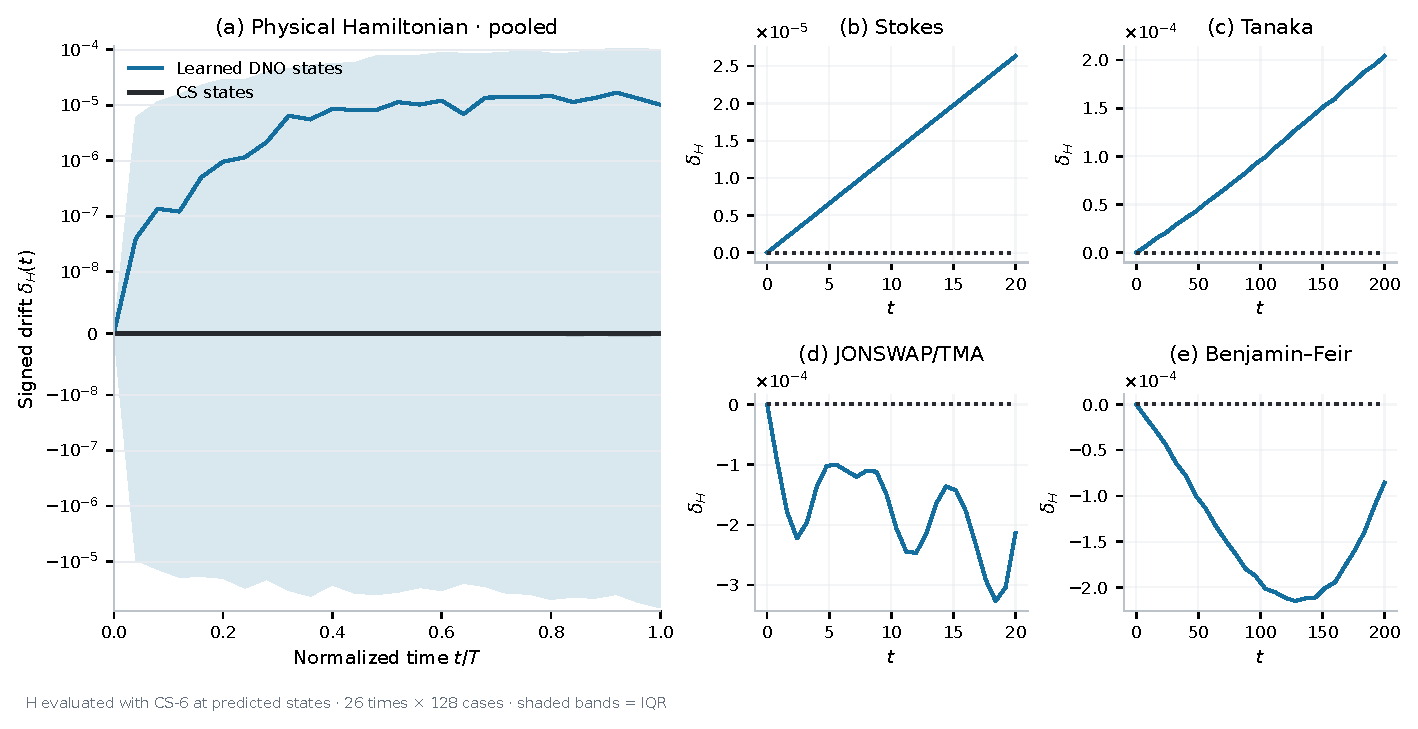
\includegraphics[width=0.98\linewidth]{07-hamiltonian-drift.pdf}
    \caption{Relative Hamiltonian drift evaluated with the reference DNO.
    Medians and interquartile ranges over 128 test cases use a symmetric-log
    scale with linear threshold $10^{-8}$; the four representative cases
    use linear axes.}
    \label{fig:hamiltonian-drift}
\end{figure}

\subsection{M-Independent Evaluation and Computational Cost}
\label{sec:TimeComp}
\subsubsection{FNO Complexity and Independence from M}
For a Craig--Sulem expansion of order $M$, the cost of one DNO evaluation is
\begin{equation}
C_{\mathrm{CS}}(N_x,M)=\Theta(M^2N_x\log N_x).
\label{eq:cs-complexity}
\end{equation}
For a one-dimensional FNO-type model with $L_\theta$ Fourier layers,
channel width $C$, and $K$ retained modes, a representative evaluation cost is
\begin{equation}
C_{\mathrm{FNO}}(N_x)=\mathcal O\!\left(
L_\theta[CN_x\log N_x+N_xC^2+KC^2]\right).
\label{eq:fno-complexity}
\end{equation}
For fixed $L_\theta,C,K$, the FNO cost is $\mathcal O(N_x\log N_x)$,
independent of $M$; this alone does not imply a wall-clock speedup.
\textcolor{blue}{Specialize this expression to the network architecture.}

Figure~\ref{fig:dno-complexity-scaling} times one DNO evaluation for a
held-out Stokes wave, Fourier-resampled to each grid. Timings exclude
compilation and use seven synchronized repeats.

\begin{figure}[tbp]
    \centering
    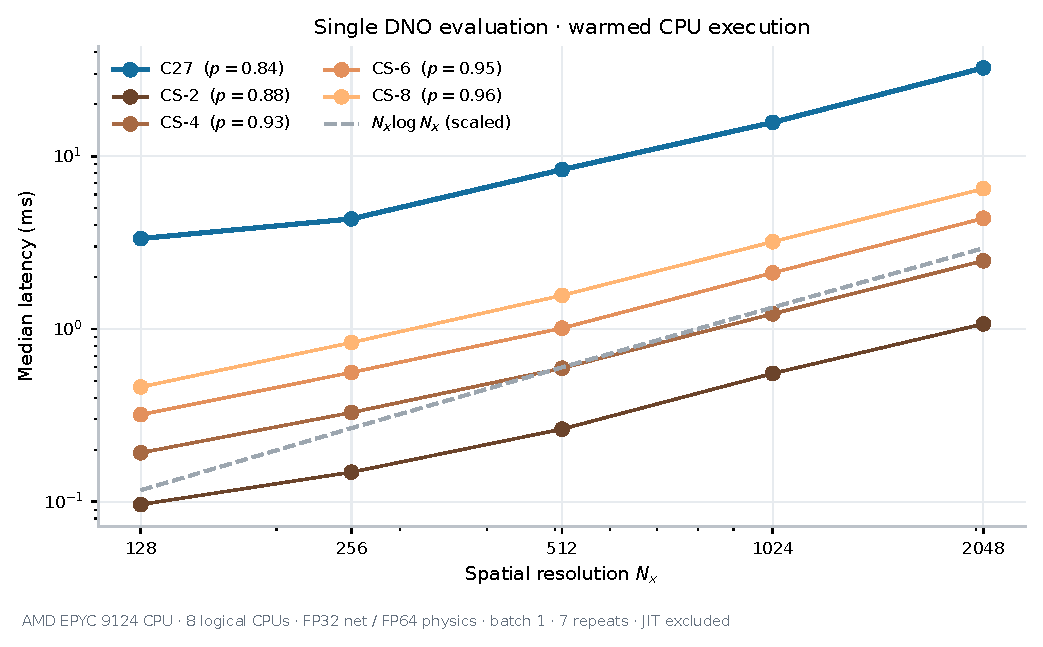
\includegraphics[width=0.92\linewidth]{08-dno-complexity-scaling.pdf}
    \caption{CPU time per DNO evaluation for the learned operator and
    Craig--Sulem orders 2, 4, 6, and 8. Curves show median times over seven
    repeats; fitted slopes describe the measured resolution range.
    A scaled $N_x\log N_x$ curve is shown for comparison.}
    \label{fig:dno-complexity-scaling}
\end{figure}

\subsubsection{Fixed-Horizon Trajectory Runtime}
For Figure~\ref{fig:runtime-tradeoff}, we integrate one held-out Stokes wave
at $N_x=256$ to $T=1$, with $\Delta t=0.01$ and a mode-64 cutoff.
Both methods use the same Gauss--Legendre integrator, four fixed-point
iterations, padding factor eight, and 51 saved states. Timings are medians
of three synchronized runs after compilation. The learned DNO is slower
than the reference series in this CPU experiment.

\begin{figure}[tbp]
    \centering
    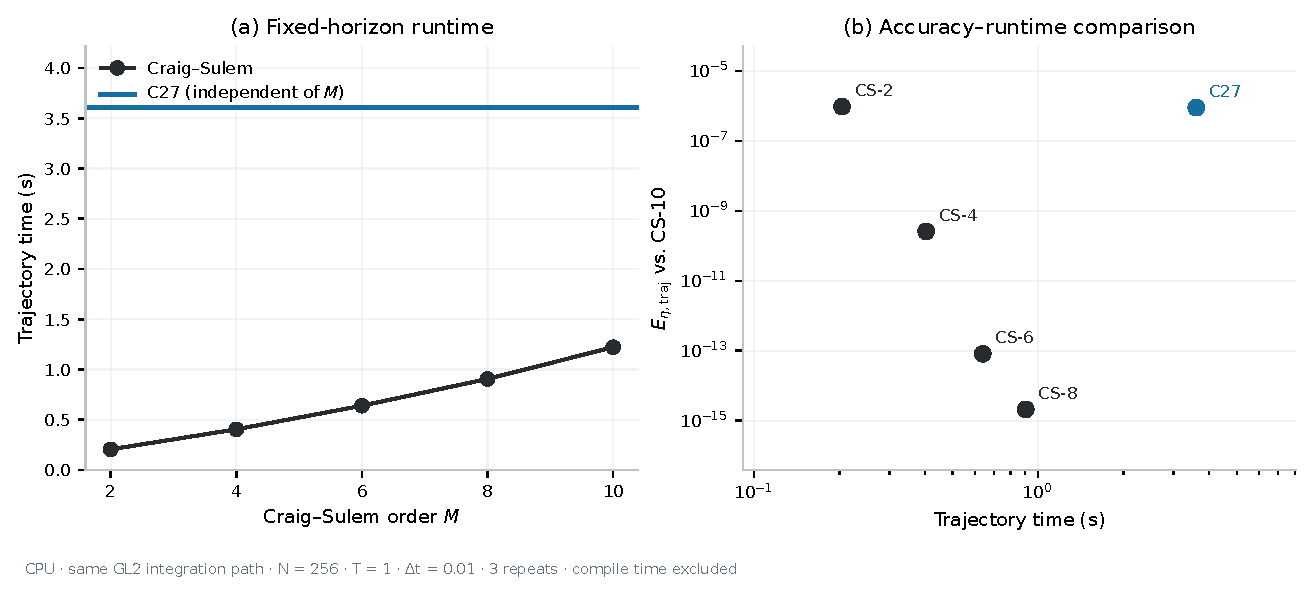
\includegraphics[width=0.98\linewidth]{09-runtime-tradeoff.pdf}
    \caption{CPU runtime and accuracy for a Stokes trajectory at
    $N_x=256$, $T=1$, and $\Delta t=0.01$. Left: runtime versus series order,
    with the learned DNO shown for comparison. Right: surface trajectory
    error relative to the order-10 reference versus runtime; its zero
    self-error is omitted from the logarithmic plot.}
    \label{fig:runtime-tradeoff}
\end{figure}

\clearpage
\section{Conclusion and Discussion}
\paragraph{Limitations}
\textcolor{blue}{Complete after the remaining comparisons.}
\paragraph{Future Work}

\section*{Acknowledgments}
This work was supported in part by\ldots

\IfFileExists{references.bib}{
    \bibliographystyle{unsrt}
    \bibliography{references}
}{
    \section*{References}
    \textcolor{blue}{Use the project's references.bib when the citations
    are completed. No bibliography file is needed to view this draft.}
}

\appendix
\section{Time-stepping Modal Error}
We demonstrate that small errors in the Fourier modes of a learned neural
surrogate for the DNO $G$ cause long-time accumulation of modal phase error
under our symplectic integration scheme.
\section{Low-Rankedness of Nonlinear Residuals of CS}
\section{More About the Dataset}
\end{document}
